\chapter{\textit{SPLINES} CÚBICAS} \label{cha:splines}

As \textit{splines} são funções definidas por partes que permitem a construção de curvas suaves a partir de um conjunto de pontos de controle. Elas são amplamente utilizadas em contextos onde é necessário representar formas complexas de maneira precisa e contínua, como na computação gráfica, modelagem geométrica e análise de dados. Dentre os diversos tipos, as \textit{splines} cúbicas se destacam por proporcionarem um bom equilíbrio entre flexibilidade e suavidade, garantindo continuidade até a segunda derivada e, consequentemente, uma transição harmoniosa entre os segmentos da curva.

Na área de biometria facial, a representação precisa das características do rosto -- como contornos dos olhos, nariz e lábios -- é essencial para o desempenho de sistemas de reconhecimento. Utilizar \textit{splines} para descrever essas formas permite capturar variações sutis da geometria facial com suavidade e fidelidade, o que é especialmente importante na comparação entre diferentes imagens. Além disso, a estrutura matemática das \textit{splines} facilita tanto a manipulação quanto a análise das curvas faciais, tornando-as uma ferramenta eficiente e robusta nesse tipo de aplicação.

Neste capítulo, serão abordadas as \textit{splines} cúbicas, suas propriedades e aplicações. A sua construção envolve a definição de um conjunto de pontos de controle e a determinação dos coeficientes que definem os polinômios cúbicos entre esses pontos. A suavidade da curva é garantida pela imposição de condições de continuidade e diferenciabilidade, resultando em uma representação suave e flexível.

\section{Definição de \textit{Splines} Cúbicas}
\label{sec:definicao-splines-cubicas}
Uma \textit{spline} cúbica é uma função definida por partes, onde cada parte é um polinômio cúbico. Dão-se, então, os polinômios de grau 3, que são especificados na forma canônica
\begin{equation}
    \vetor{p}(t) = \vetor{c_0} + \vetor{c_1}t + \vetor{c_2}t^2 + \vetor{c_3}t^3,
\end{equation}
onde $t$ é o parâmetro de interpolação e cada $\vetor{c_i}$ é um vetor no $\mathbb{R}^2$. A função $\vetor{p}(t)$ representa uma curva parametrizada com variável independente \( t \in [0,1] \). Essa função descreve a posição ao longo da curva no plano bidimensional, sendo essa posição o elemento de interesse ao desenharmos a curva, já que o processo de plotagem envolve a determinação de pontos com coordenadas $(x, y)$. Em outras palavras, as splines cúbicas são definidas por equações paramétricas, ou seja, ambas as componentes $x$ e $y$ são expressas como funções da variável $t$.

As curvas de Hermite são uma forma alternativa de representar curvas cúbicas. Expressar uma curva cúbica na forma de Hermite consiste em fornecer quatro valores fundamentais -- conhecidos como valores de Hermite -- que contêm todas as informações necessárias para descrever completamente a curva. Esses valores também permitem calcular os coeficientes da variável \( t \) na equação polinomial cúbica padrão, resultando assim na expressão completa da curva como um polinômio.

A principal motivação para utilizar a forma de Hermite está na possibilidade de determinar os coeficientes do polinômio diretamente a partir de informações conhecidas: a posição do ponto inicial da curva, \( \vetor{p_0} = \vetor{p}(0) \); a posição do ponto final, \( \vetor{p_1} = \vetor{p}(1) \); além das tangentes nesses pontos, ou seja, a taxa de variação da curva em \( \vetor{p_0} \), denotada por \( \vetor{v_0} = \vetor{v}(0) \), e em \( \vetor{p_1} \), denotada por \( \vetor{v_1} = \vetor{v}(1) \).


Agora que se conhecem os valores de Hermite, é possível resolvê-los através do sistema de equações
\begin{align}
    \vetor{p}(0) &= \vetor{c_0} + \vetor{c_1}(0) + \vetor{c_2}(0)^2 + \vetor{c_3}(0)^3 = \vetor{c_0}, \\
    \vetor{p}(1) &= \vetor{c_0} + \vetor{c_1} + \vetor{c_2} + \vetor{c_3}.
\end{align}
Para encontrar $v_0$ e $v_1$ é necessário calcular a derivada da posição. Portanto
\begin{align}
    \vetor{v}(t) &= \dfrac{d}{dt}\vetor{p}(t) = \vetor{c_1} + 2\vetor{c_2}t + 3\vetor{c_3}t^2,\\
    \vetor{v}(0) &= \vetor{c_1},\\
    \vetor{v}(1) &= \vetor{c_1} + 2\vetor{c_2} + 3\vetor{c_3}.
\end{align}
Então é possível obter a fórmula
\begin{align}
    \vetor{c_0} &= \vetor{p_0},\\
    \vetor{c_1} &= \vetor{v_0},\\
    \vetor{c_2} &= -3\vetor{p_0} - 2\vetor{v_0} - \vetor{v_1} + 3\vetor{p_1},\\
    \vetor{c_3} &= 2\vetor{p_0} + \vetor{v_0} + \vetor{v_1} - 2\vetor{p_1}. 
\end{align}
Escrevendo na forma matricial de Hermite, é obtida a expressão
\begin{equation}
    \vetor{p}(t) =  
        \left(
        \begin{array}{rrrr}
            1 & t & t^2 & t^3
        \end{array}\right)
        \left(
        \begin{array}{rrrr}
            1 & 0 & 0 & 0 \\
            0 & 0 & 1 & 0 \\
            -3 & 3 & -2 & -1 \\
                2 & -2 & 1 & 1
        \end{array}\right)
    \left(
        \begin{array}{r}
            \vetor{p_0} \\
            \vetor{p_1} \\
            \vetor{v_0} \\
            \vetor{v_1}
        \end{array}\right).
 \end{equation}

 \subsection{Criação da \textit{Spline}}

 Supondo que existam 4 pontos e é desejado criar uma \textit{spline} que passe por todos eles, é necessário criar 3 segmentos de curvas cúbicas, cada uma passando por dois pontos consecutivos. Assim, a \textit{spline} será composta por 3 segmentos cúbicos, cada um definido por 4 pontos de controle \cite{CatmullRom}.

 A primeira curva irá de $\vetor{p_0}$ a $\vetor{p_1}$, a segunda de $\vetor{p_1}$ a $\vetor{p_2}$ e a final de $\vetor{p_2}$ a $\vetor{p_3}$. Então é aplicada a fórmula que foi derivada acima para $\vetor{p_t}$, mas em 3 variantes diferentes, cada variante com um par diferente de pontos iniciais e finais. A fórmula da primeira curva terá pontos iniciais e finais $\vetor{p_0}$ e $\vetor{p_1}$, a segunda em $\vetor{p_1}$ e $\vetor{p_2}$ e a terceira em $\vetor{p_2}$ e $\vetor{p_3}$, como é possível ver na \autoref{fig:spline_tangentes}. No que diz respeito às tangentes, \citet{CatmullRom} propuseram uma abordagem baseada na diferença entre pontos adjacentes: a tangente em um ponto pode ser obtida subtraindo-se o ponto anterior do ponto seguinte. Por exemplo, a tangente no ponto $\vetor{p_2}$ é dada por $\vetor{p_3} - \vetor{p_1}$. É comum, ainda, dividir esse resultado por 2, pois essa operação tende a produzir curvas visualmente mais suaves e esteticamente agradáveis. Logo, é possível reescrever a equação em termos de quatro pontos ($\vetor{p_0}$ a $\vetor{p_3}$).


\begin{figure}[h!]
    \caption{CURVAS CÚBICAS DE CATMULL-ROM.}
    \centering
    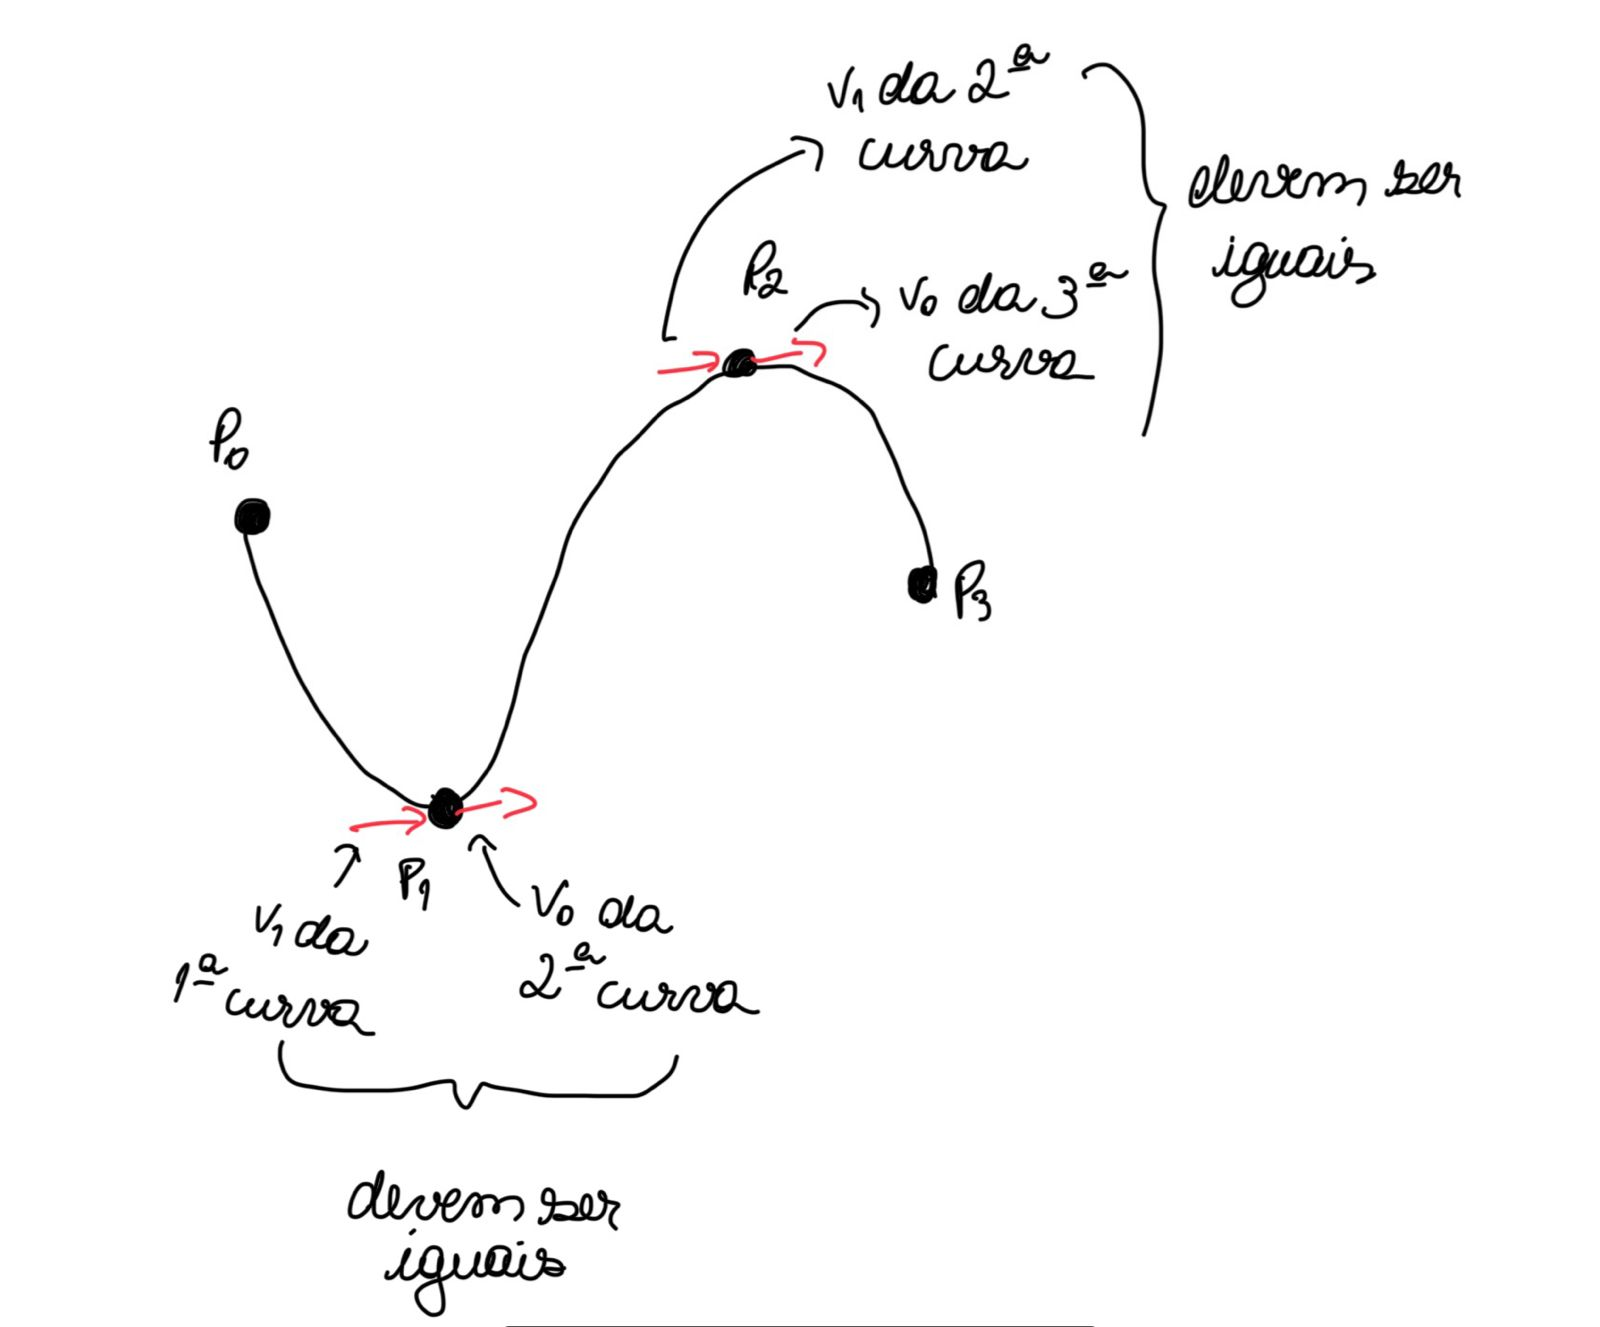
\includegraphics[width=0.8\textwidth]{fig/s1.jpg}
    \legend{\textit{Spline} cúbica com 4 pontos de controle}
    \vspace{0.5em} % Espaçamento vertical entre as imagens
    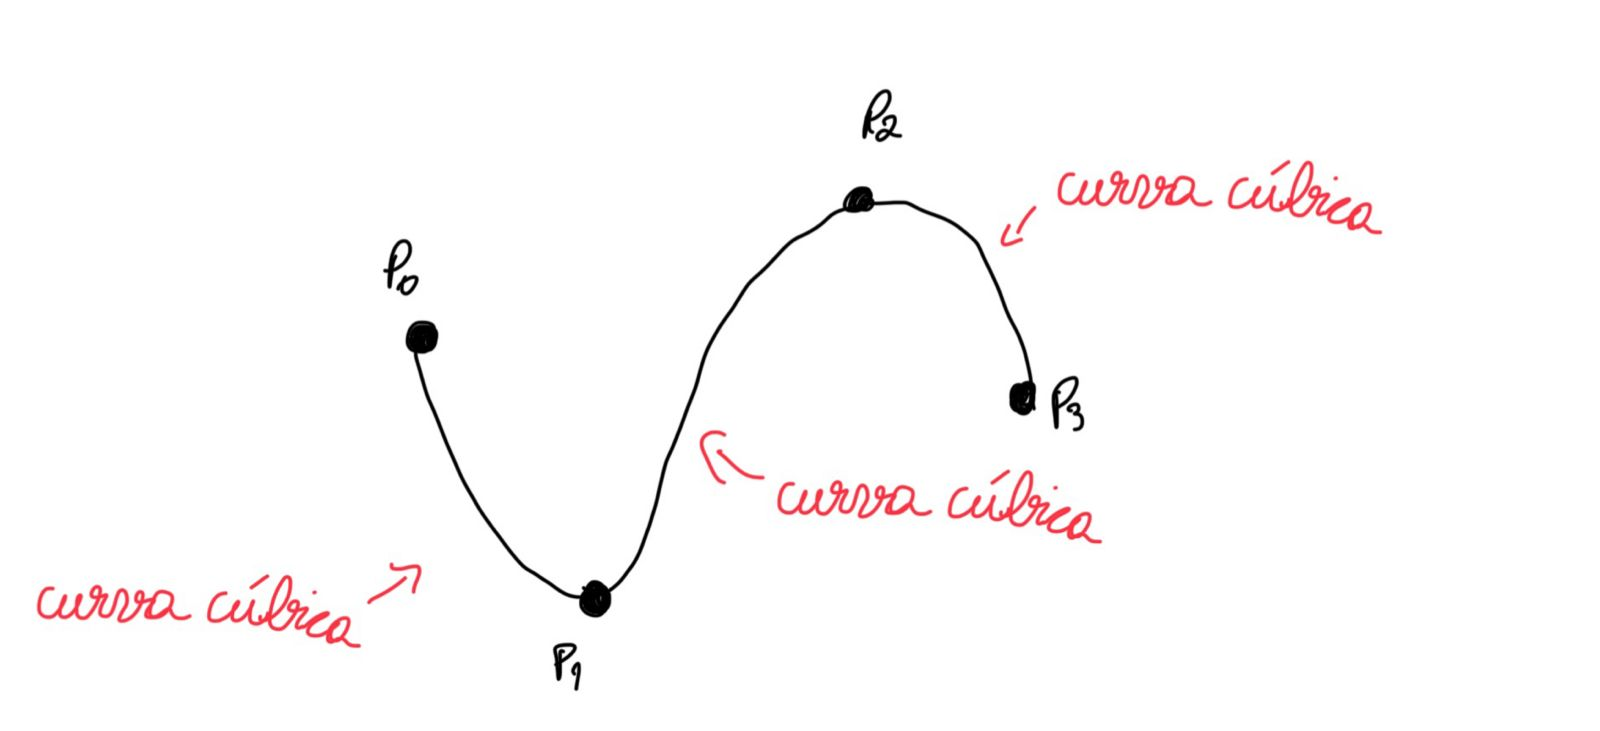
\includegraphics[width=0.8\textwidth]{fig/s2.jpg}
    \legend{Tangentes coincidentes nas conexões das cúbicas em cada ponto.}
    \legend{FONTE: A autora.}
    \label{fig:spline_tangentes}
\end{figure}


Outra complicação que surge é que, ao se utilizar o ponto anterior e o ponto seguinte para o cálculo das tangentes, surge a dúvida sobre qual deve ser considerado o ponto anterior ao ponto inicial, $\vetor{p_i}$, e o ponto seguinte ao ponto final, $\vetor{p_f}$. Uma solução comum para esse problema é a adição de \textit{pontos fantasmas}, que não fazem parte da curva, mas são utilizados apenas para o cálculo das tangentes.


Então ficamos com
\begin{equation}
    \vetor{p}(t) =  
        \left(
        \begin{array}{rrrr}
            1 & t & t^2 & t^3
        \end{array}
        \right)
        \left(
        \begin{array}{rrrr}
            1 & 0 & 0 & 0 \\
            0 & 0 & 1 & 0 \\
            -3 & 3 & -2 & -1 \\
                2 & -2 & 1 & 1
        \end{array}
        \right)
    \left(
        \begin{array}{r}
            \vetor{p_1} \\
            \vetor{p_2} \\
            \frac{\vetor{p_2} - \vetor{p_0}}{2\tau} \\
                \frac{\vetor{p_3} - \vetor{p_1}}{2\tau}
        \end{array}
        \right),
\end{equation}
onde $\tau$ é um fator de escala que pode ser ajustado para controlar a suavidade da curva. O valor de $\tau$ pode ser definido com base na distância entre os pontos de controle ou em outras considerações geométricas. Com isso é possível chegar no formato de Catmull-Rom
\begin{equation}
    \vetor{p}(t) = \frac{1}{2}
       \left(
 	\begin{array}{rrrr}
 		1 & t & t^2 & t^3
 	\end{array}
    \right)
    \left(
 	\begin{array}{rrrr}
 		0 & 2 & 0 & 0 \\
 	    -\tau & 0 & \tau & 0 \\
 		2\tau & \tau-6 & -2(\tau-3) & -\tau \\
            -\tau & 4-\tau & \tau-4 & \tau
 	\end{array}
    \right)
   \left(
 	\begin{array}{r}
 		\vetor{p_0} \\
 	    \vetor{p_1} \\
 		\vetor{p_2} \\
            \vetor{p_3}
 	\end{array}
    \right).
\end{equation}

Na \autoref{fig:tensao} é possível observar que quanto menor a tensão $\tau$, menos suave fica a curva.

\begin{figure}[h!]
    \caption{TENSÃO DA CURVA.}
    \centering
    \begin{minipage}[b]{0.45\textwidth}
        \centering
        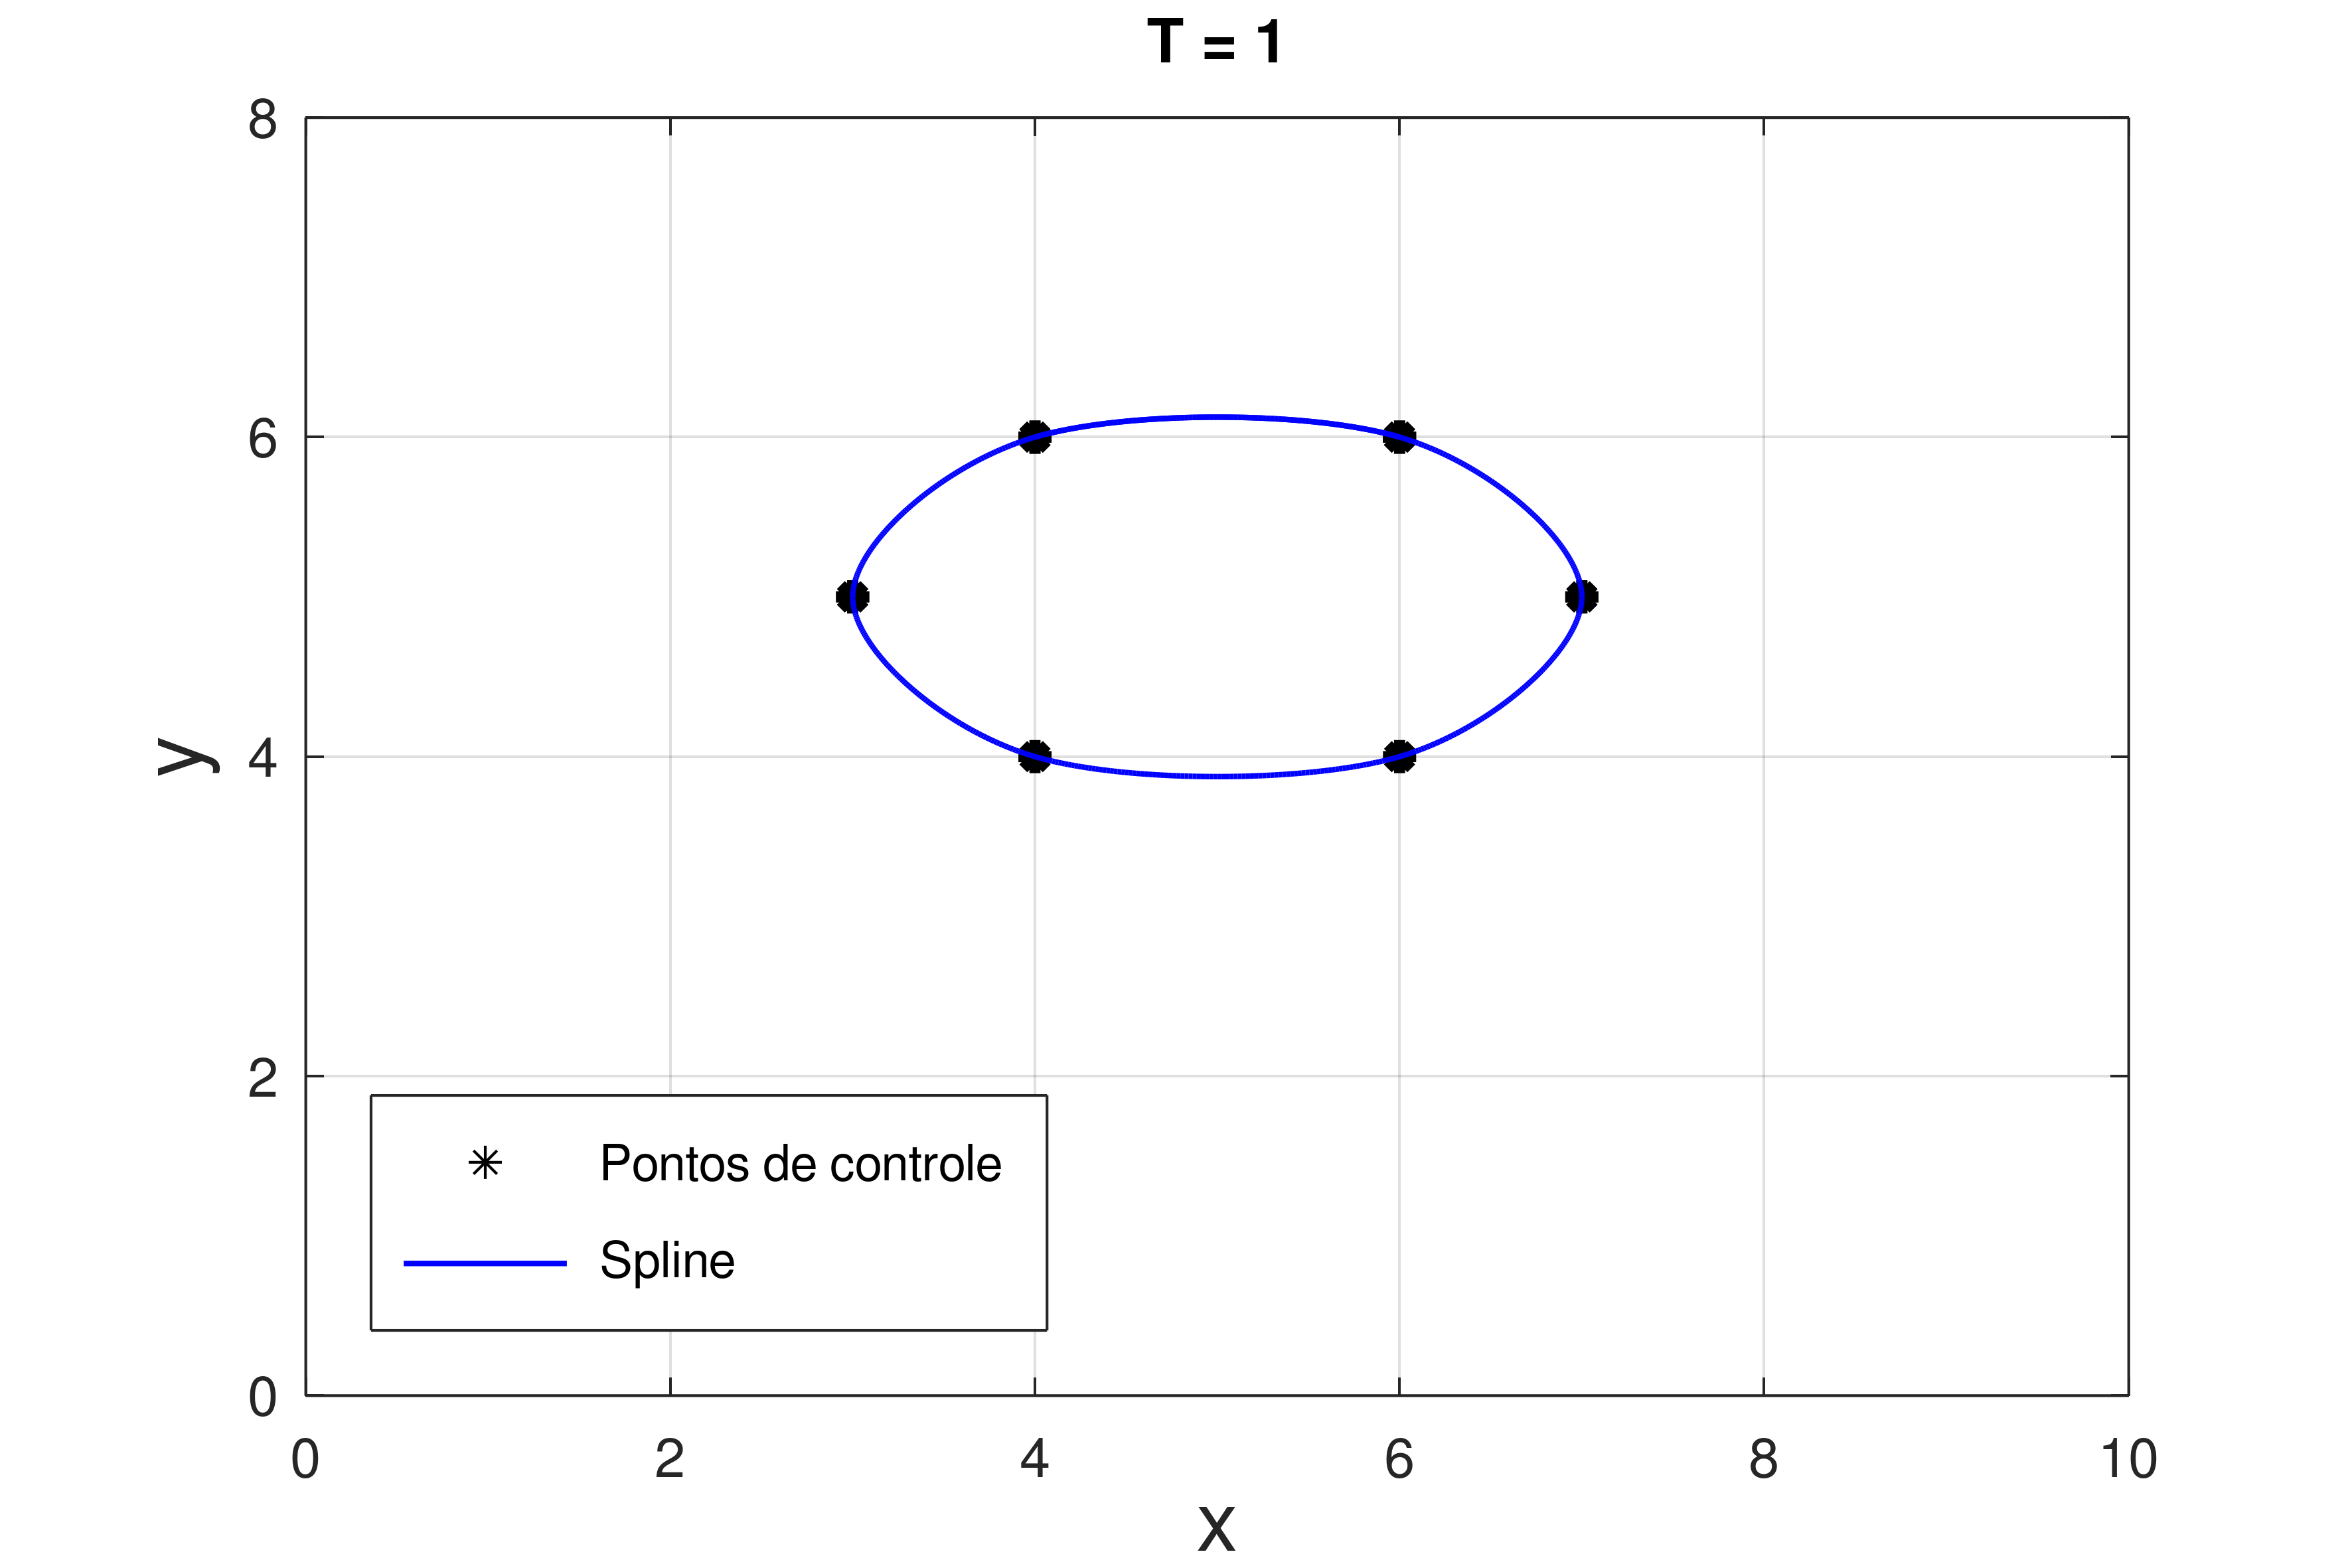
\includegraphics[width=1\linewidth]{fig/cat_rom_t1.png}
        \legend{$\tau$ = 1.}
        \label{fig:tesao1}
    \end{minipage}
    \hfill
    \begin{minipage}[b]{0.45\textwidth}
        \centering
        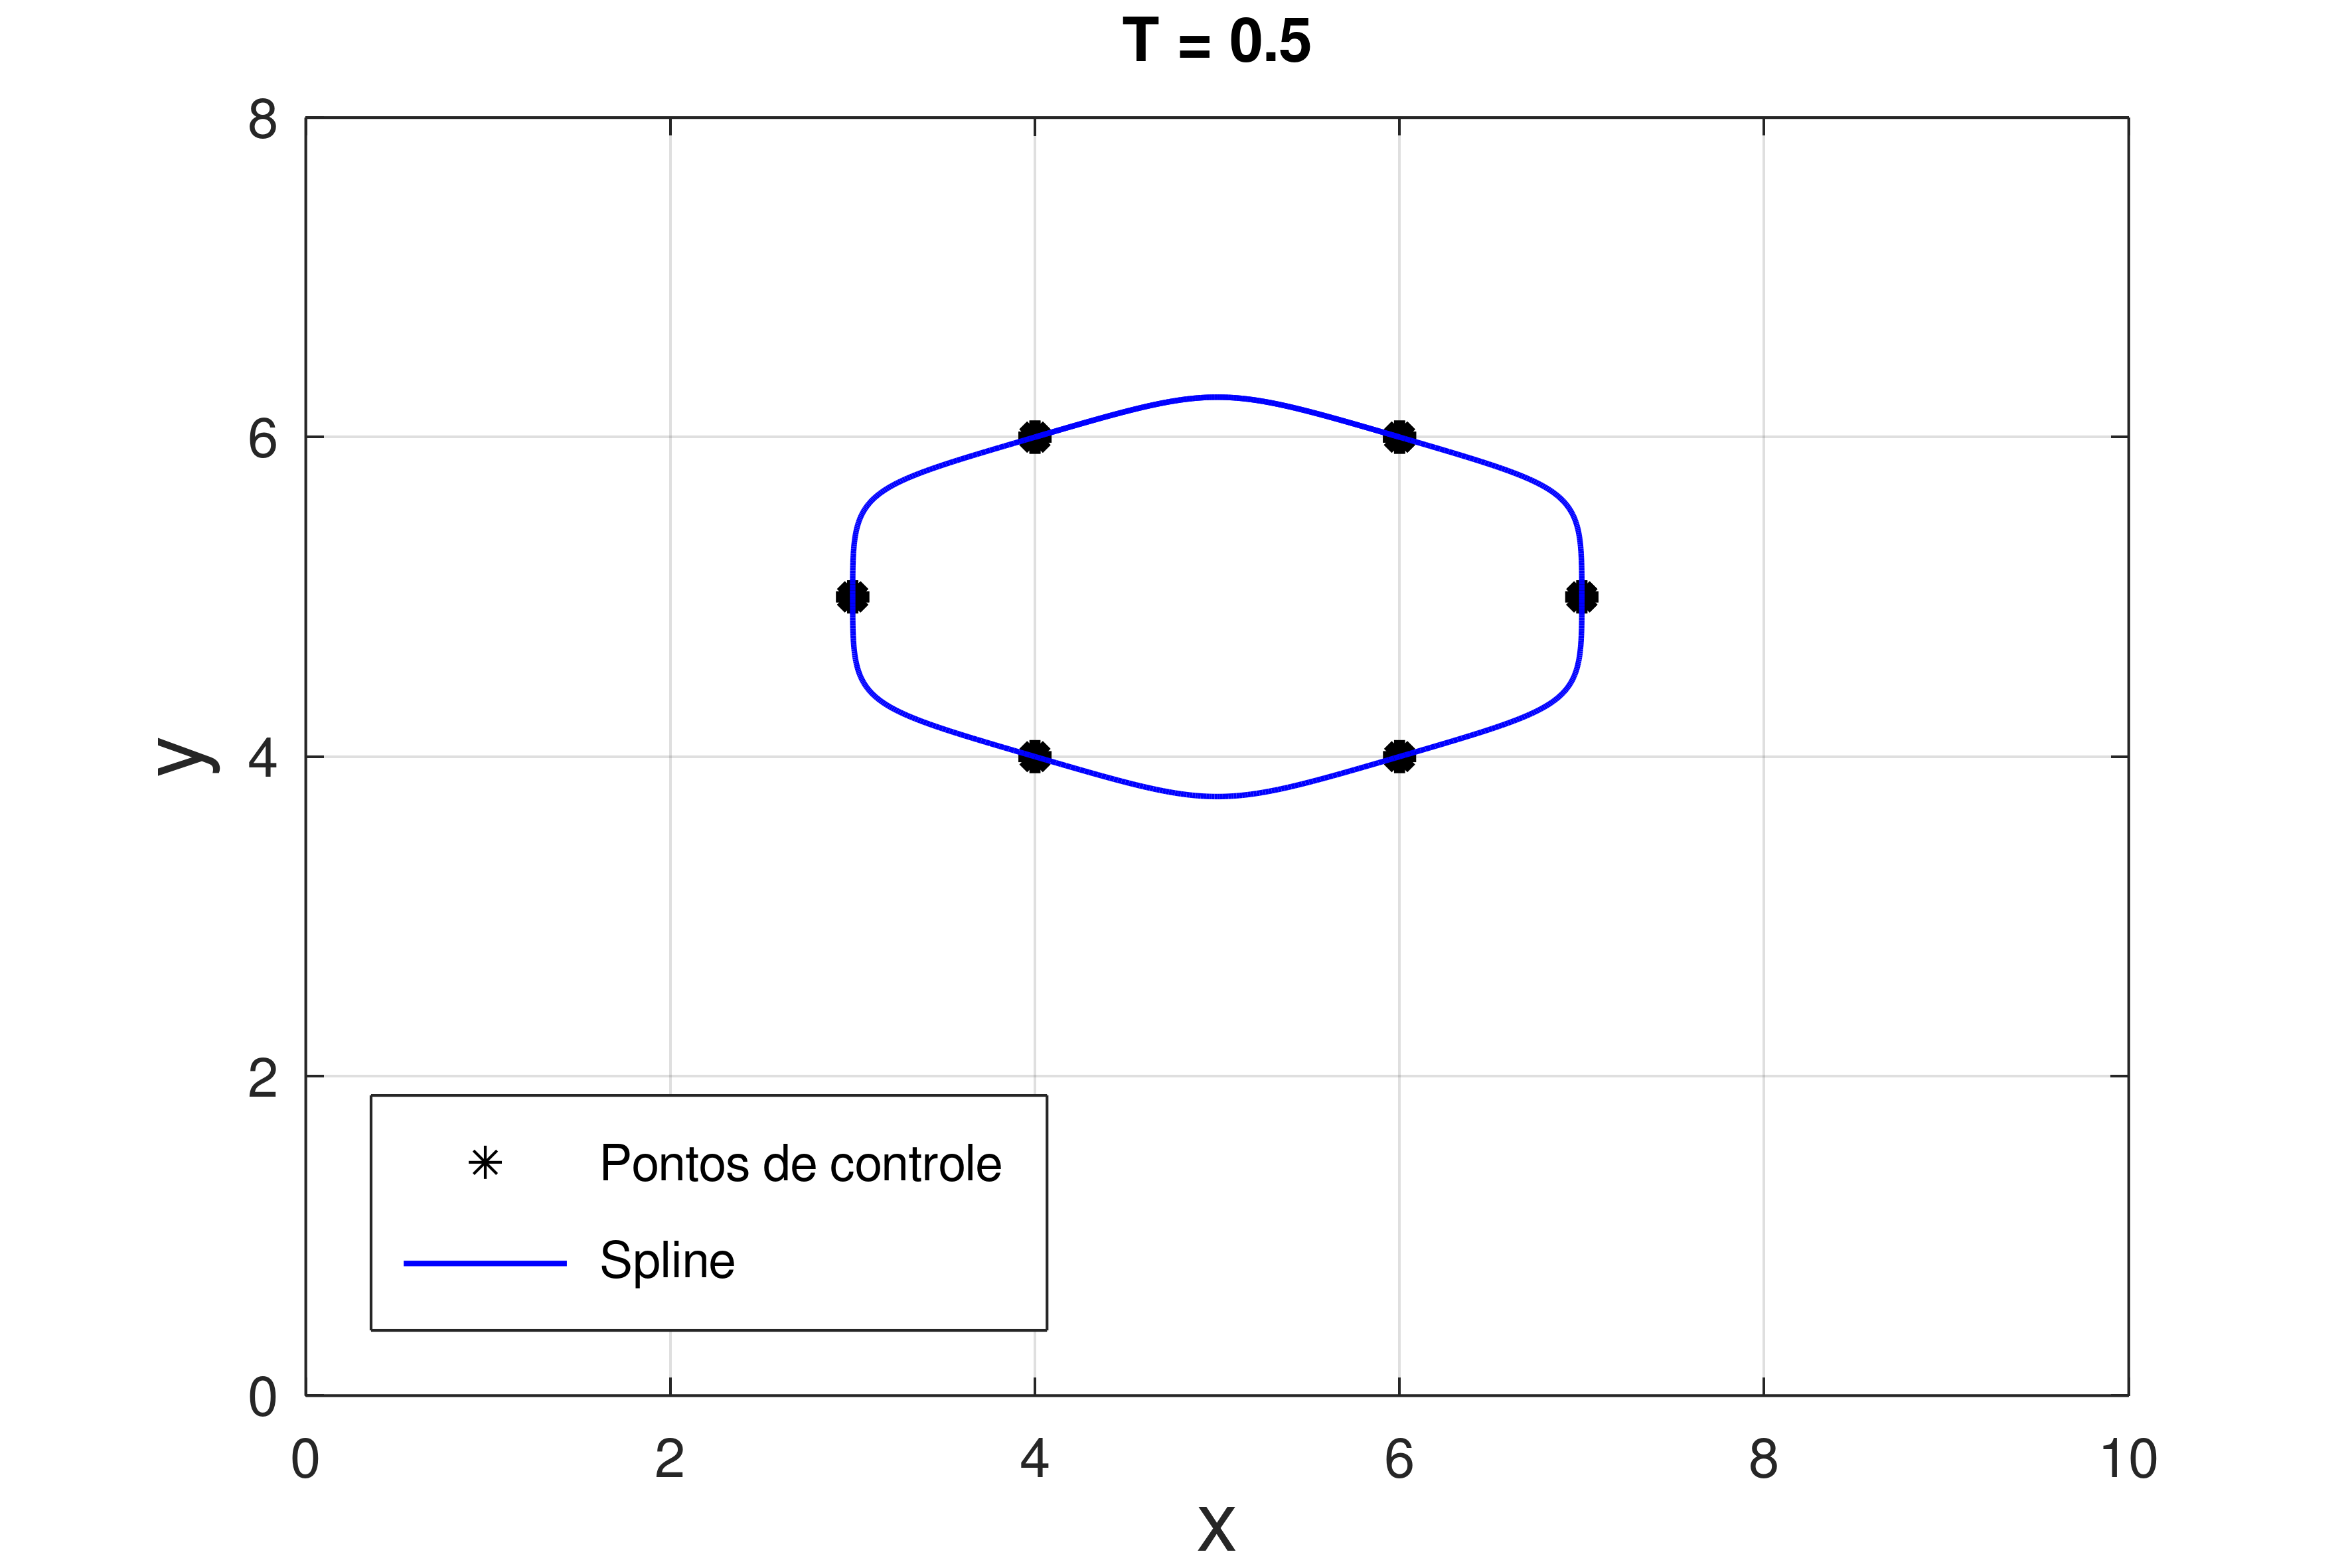
\includegraphics[width=1\linewidth]{fig/cat_rom_t05.png}
        \legend{$\tau$ = 0.5.}
        \label{fig:tensao05}
    \end{minipage}

    \vspace{1cm}

    \begin{minipage}[b]{0.45\textwidth}
        \centering
        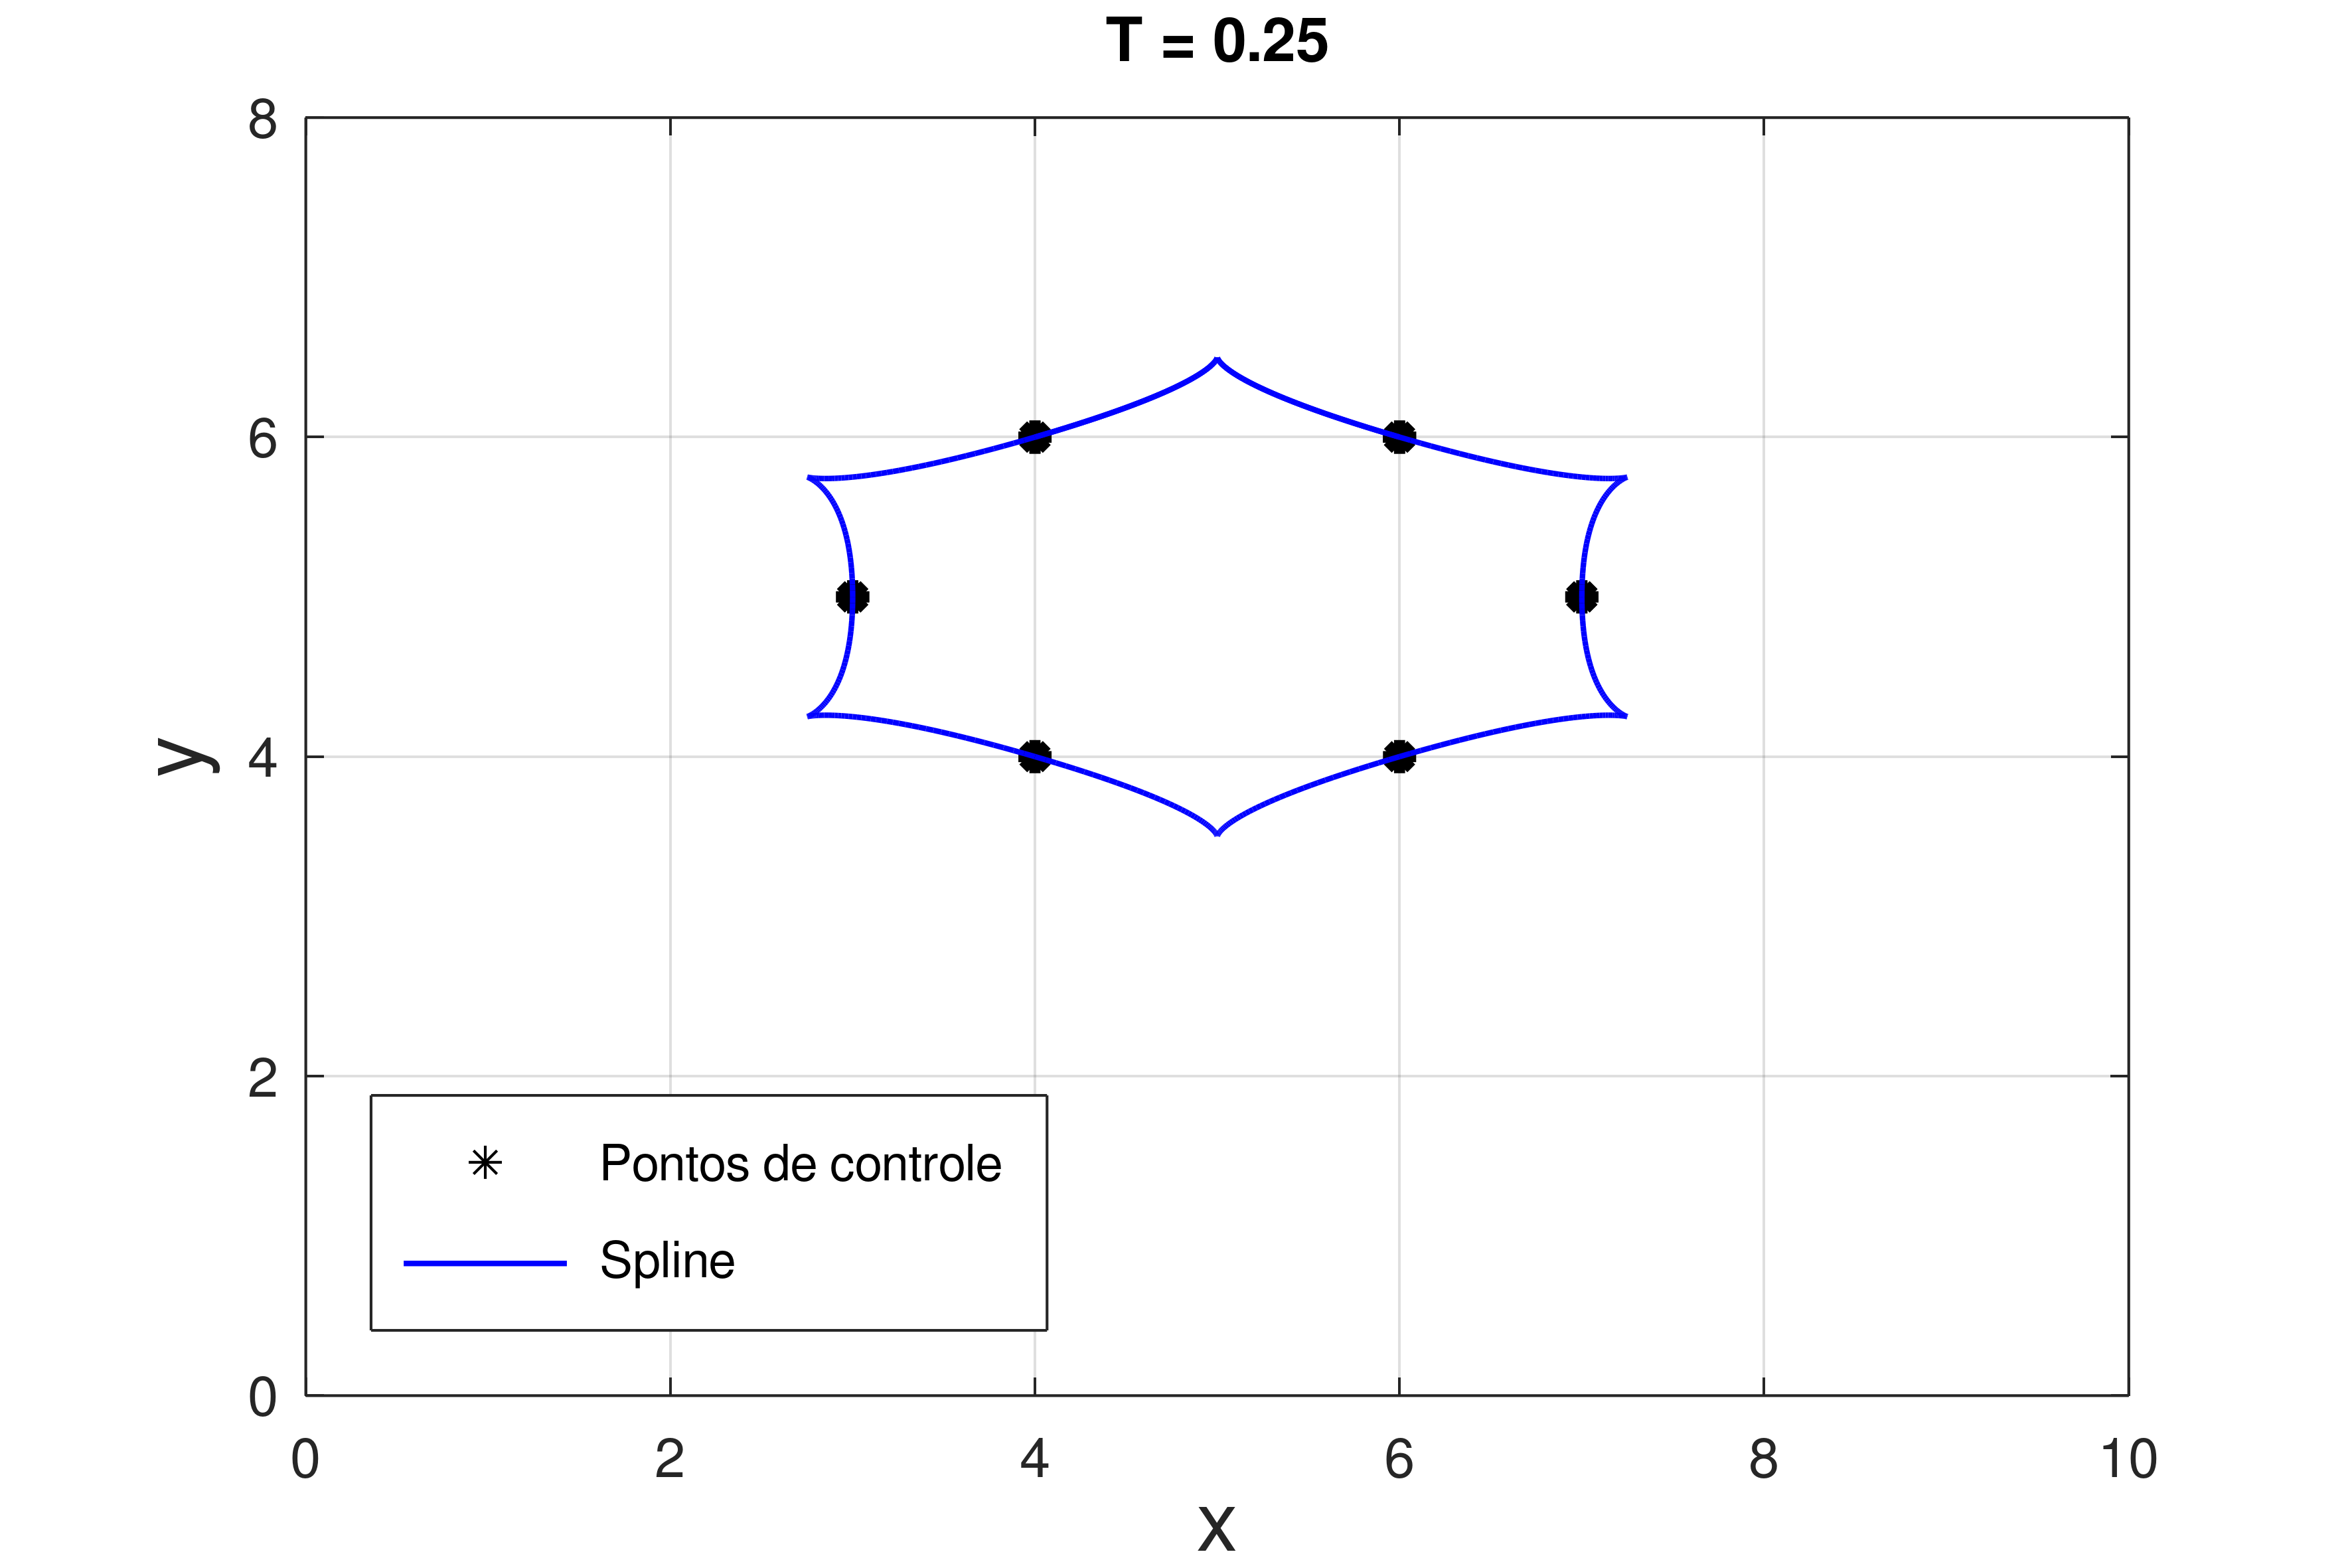
\includegraphics[width=1\linewidth]{fig/cat_rom_t025.png}
        \legend{$\tau$ = 0.25.}
        \label{fig:tensao025}
    \end{minipage}
    \label{fig:tensao}
    \legend{FONTE: A autora.}
\end{figure}

\subsection{Resultados}

Foi implementado um algoritmo autoral que gera uma \textit{spline} cúbica a partir de um conjunto de pontos de controle. O algoritmo proposto utiliza a fórmula de Catmull-Rom para calcular os coeficientes da curva, garantindo suavidade e continuidade. 

A \autoref{fig:splines_resultados} apresenta os resultados obtidos a partir de conjuntos de pontos de controle extraídos da imagem, conforme o processo descrito no \autoref{cha:processamento-imagem}. É importante ressaltar que os pontos foram reordenados de modo a garantir que a curva resultante seja traçada sempre da esquerda para a direita, o que é essencial para o bom desempenho do algoritmo de DTW.


\begin{figure}[h!]
    \caption{\textit{SPLINES} NOS PONTOS EXTRAÍDOS.}
    \centering
    \begin{minipage}[b]{0.45\textwidth}
        \centering
        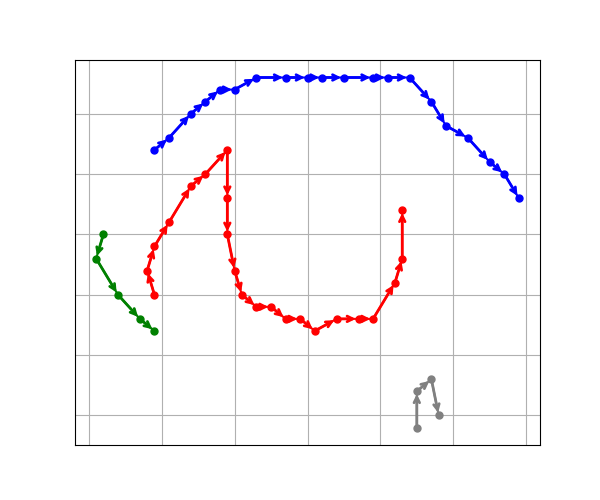
\includegraphics[width=1\linewidth]{fig/07_sorted_points_right_eye.png}
        \legend{Reordenação dos pontos.}
        \label{fig:reordenacao}
    \end{minipage}
    \hfill
    \begin{minipage}[b]{0.45\textwidth}
        \centering
        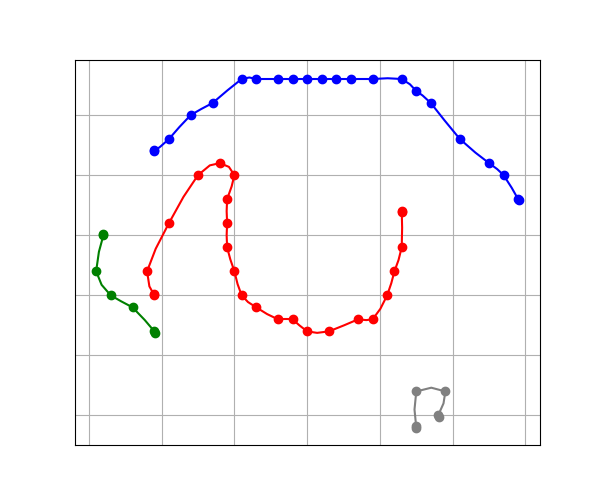
\includegraphics[width=1\linewidth]{fig/08_spline_plot_right_eye.png}
        \legend{\textit{Splines}.}
        \label{fig:spline}
    \end{minipage}
    \label{fig:splines_resultados}
    \legend{FONTE: A autora.}
\end{figure}





% \begin{algorithm}[H]
%     \renewcommand{\algorithmcfname}{Algoritmo}%
%     \SetAlgoLined
%     \eSe{$n\leq r$}{
%         Calcule a fatoração $\vetor{M}=\vetor{LU}$ por outro método\;
%     }{
%         Calcule a fatoração $\left[\begin{array}{cc} \vetor{A}\\\vetor{C}\end{array}\right]=\left[\begin{array}{cc} \vetor{L_{11}}\\\vetor{L_{21}}\end{array}\right]\vetor{U_{11}}$\;
%         Calcule $\vetor{U_{12}}=\vetor{L_{11}^{-1}}\vetor{B}$ pela solução do sistema linear $\vetor{L_{11}}\vetor{U_{12}}=\vetor{B}$\;
%         $\vetor{\tilde{D}} \gets \vetor{D}-\vetor{L_{21}}\vetor{U_{12}}$\;
%         Calcule a fatoração $\vetor{\tilde{D}}=\vetor{L_{22}}\vetor{U_{22}}$ recursivamente\;
%         Retorne $\vetor{L}=\left[\begin{array}{cc} \vetor{L_{11}} & \vetor{0}\\\vetor{L_{21}} & \vetor{L_{22}}\end{array}\right]$ e $\vetor{U}=\left[\begin{array}{cc} \vetor{U_{11}} & \vetor{U_{12}}\\\vetor{0} & \vetor{U_{22}}\end{array}\right]$\;
%     }
% \end{algorithm}

% \begin{algorithm}
%     \caption{Fatoração QR magra de uma matriz $\vetor{A}\in\R^{m\times n}$ usando Gram-Schmidt.}
%     \SetAlgoLined
%     \Para{$k$ de $1$ até $n$}{
%         $\vetor{v_k} \gets \vetor{A}[:,k]$\;
%         \Para{$i$ de $1$ até $k-1$}{
%             $\vetor{R}[i,k] \gets \vetor{Q}[:,i]^{\vetor{T}}\vetor{A}[:,k]$\;
%             $\vetor{v_k} \gets \vetor{v_k}-\vetor{R}[i,k]\vetor{Q}[:,i]$\;
%         }
%         $\vetor{R}[k,k]\gets\left\|\vetor{v_k}\right\|_2$\;
%         $\vetor{Q}[:,k]\gets\dfrac{1}{\vetor{R}[k,k]}\vetor{v_k}$\;
%     }
%     \label{alg:QRmagra}
% \end{algorithm}